\documentclass{article}
\usepackage[utf8]{inputenc}
\usepackage[T1]{fontenc}
\usepackage[french]{babel}
\usepackage{graphicx}

\title{Rendu n.1 Projet technologique}
\author{Zoé Debaty}
\date{November 2019}

\begin{document}

\maketitle
\tableofcontents 
\newpage

% Spécificités techniques %
\section{Spécificités techniques}

% L'image %
\subsection{L'image}
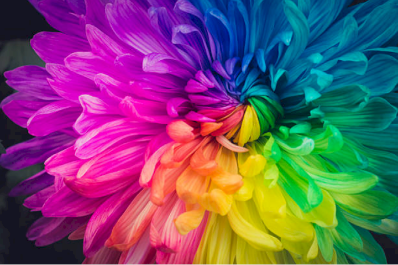
\includegraphics[width=10cm]{../multicolor}

\begin{itemize}
\item Nom : "multicolor"
\item Dimensions : 612p * 408p
\item Taille : 59,9 Ko
\end{itemize}
\medbreak

L'image à été choisie car elle possède des changements de luminosité et énorméments de couleurs afin de tester au mieux mes fonctions.

% Le telephone %
\subsection{Le téléphone}

Pour tester mes fonctions j'utilise un Sony Xpéria XA, avec une définition d'écran de 1280 * 720 et une diagonale de 5 pouces.\\
Il tourne sous Android Nougat 7.0.

\newpage

% Functions %
\section{Fonctions}

% Saturation %
\subsection{Saturation}
Cette fonction permet de modifier la saturation de l'image en ajoutant/enlevant des pourcentages (10\%) à l'image HSV.
\bigbreak

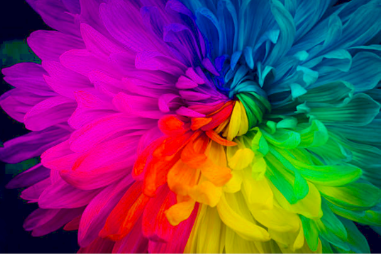
\includegraphics[width=10cm]{../SaturationMax}

Image de base avec la saturation au maximum.
\bigbreak

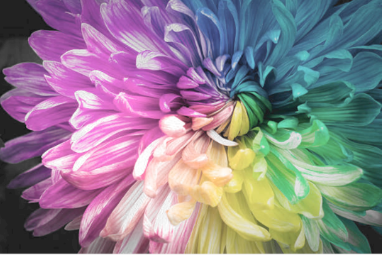
\includegraphics[width=10cm]{../SaturationMoins6}

Image de base avec 60\% de saturation en moins.

% Luminosite %
\subsection{Luminosité}
Cette fonction permet de changer la luminosité de l'image en ajoutant/enlevant des pourcentages (10\%) à l'image HSV.
\bigbreak

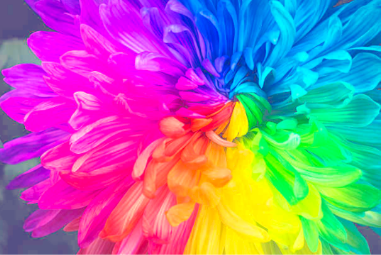
\includegraphics{../LuminositePlus3}

Image de base avec 30\% de luminosité en plus.
\bigbreak

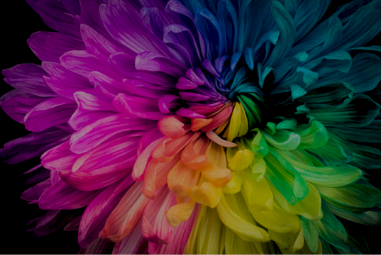
\includegraphics{../LuminositeMoins3}

Image de base avec 30\% de luminosité en moins.

% Selection de couleurs %
\subsection{Selection de couleurs \underline{TD 2 Qestion 2.2}}

Cette fonction permet, au moyen de deux limites (qu'on modifie de 10 en 10), d'afficher ou non certaines couleurs.
\bigbreak

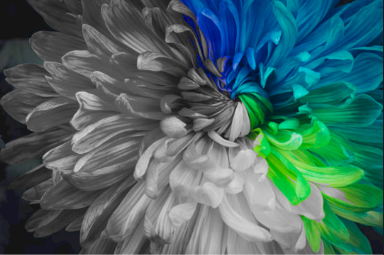
\includegraphics{../SelectedColor}

Image de base avec les deux limites n'affichants que les parties bleus et vertes de l'image.

% Negatif %
\subsection{Negatif}
Cette fonction passe l'image en négatif.
\bigbreak

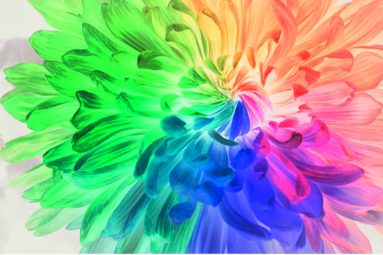
\includegraphics{../Negatif}

Image de base en négatif

% Extension linéaire %
\subsection{Extension linéaire \underline{TD 3 Qestion 1.1}}
Cette fonction est l'implémentation de 

% Version grise %
\subsection{Version grise \underline{TD 1 Question 3}}

% Couleur aleatoir %
\subsection{Couleur aléatoire \underline{TD 2 Question 2.1}}

\end{document}
